
\documentclass[letterpaper,hide notes,xcolor={table,svgnames},pdftex,10pt]{beamer}
\def\showexamples{t}

\usecolortheme{crane}
\setbeamertemplate{navigation symbols}{}

\usetheme{MyPittsburgh}
\usepackage{hyperref}
\usepackage{graphicx,xspace}
\usepackage[normalem]{ulem}
\usepackage{multicol}
\usepackage{amsmath,amssymb,amsthm,graphicx,xspace}
\newcommand\SF[1]{$\bigstar$\footnote{SF: #1}}

\usepackage[sfdefault,lf]{carlito}
\usepackage[T1]{fontenc}
\usepackage[scaled]{beramono}
\usepackage{tikzpagenodes}
\newcommand{\Rplus}{\protect\hspace{-.1em}\protect\raisebox{.35ex}{\small{\small\textbf{+}}}}
\newcommand{\Cpp}{\mbox{C\Rplus\Rplus}\xspace}

\newcounter{tmpnumSlide}
\newcounter{tmpnumNote}

\newcommand\mnote[1]{%
	\addtocounter{tmpnumSlide}{1}
	\ifdefined\showcues {~\tiny\fbox{\arabic{tmpnumSlide}}}\fi
	\note{\setlength{\parskip}{1ex}\addtocounter{tmpnumNote}{1}\textbf{\Large \arabic{tmpnumNote}:} {#1\par}}}

\newcommand\mmnote[1]{\note{\setlength{\parskip}{1ex}#1\par}}


\newcommand\mquestion[2]{{~\color{red}\fbox{?}}\note{\setlength{\parskip}{1ex}\par{\Large \textbf{?}} #1} \note{\setlength{\parskip}{1ex}\par{\Large \textbf{A}} #2\par}\ifdefined \presentationonly \pause \fi}

\newcommand\blackboard[1]{%
	\ifdefined   \showblackboard
		{#1}
	\else {\begin{center} \fbox{\colorbox{blue!30}{%
						\begin{minipage}{.95\linewidth}%
							\hspace{\stretch{1}} Some space intentionally left blank; done at the blackboard.%
						\end{minipage}}}\end{center}}%
	\fi%
}

\usepackage{listings}
\lstset{%
	keywordstyle=\bfseries,
	aboveskip=15pt,
	belowskip=15pt,
	captionpos=b,
	identifierstyle=\ttfamily,
	frame=lines,
	numbers=left, basicstyle=\scriptsize, numberstyle=\tiny, stepnumber=0, numbersep=2pt}

\usepackage{siunitx}
\newcommand\sius[1]{\num[group-separator = {,}]{#1}\si{\micro\second}}
\newcommand\sims[1]{\num[group-separator = {,}]{#1}\si{\milli\second}}
\newcommand\sins[1]{\num[group-separator = {,}]{#1}\si{\nano\second}}
\sisetup{group-separator = {,}, group-digits = true}

%% -------------------- tikz --------------------
\usepackage{tikz}
\usetikzlibrary{positioning}
\usetikzlibrary{arrows,backgrounds,automata,decorations.shapes,decorations.pathmorphing,decorations.markings,decorations.text}

\tikzstyle{place}=[circle,draw=blue!50,fill=blue!20,thick, inner sep=0pt,minimum size=6mm]
\tikzstyle{transition}=[rectangle,draw=black!50,fill=black!20,thick, inner sep=0pt,minimum size=4mm]

\tikzstyle{block}=[rectangle,draw=black, thick, inner sep=5pt]
\tikzstyle{bullet}=[circle,draw=black, fill=black, thin, inner sep=2pt]

\tikzstyle{pre}=[<-,shorten <=1pt,>=stealth',semithick]
\tikzstyle{post}=[->,shorten >=1pt,>=stealth',semithick]
\tikzstyle{bi}=[<->,shorten >=1pt,shorten <=1pt, >=stealth',semithick]

\tikzstyle{mut}=[-,>=stealth',semithick]

\tikzstyle{treereset}=[dashed,->, shorten >=1pt,>=stealth',thin]

\usepackage{ifmtarg}
\usepackage{xifthen}
\makeatletter
% new counter to now which frame it is within the sequence
\newcounter{multiframecounter}
% initialize buffer for previously used frame title
\gdef\lastframetitle{\textit{undefined}}
% new environment for a multi-frame
\newenvironment{multiframe}[1][]{%
	\ifthenelse{\isempty{#1}}{%
		% if no frame title was set via optional parameter,
		% only increase sequence counter by 1
		\addtocounter{multiframecounter}{1}%
	}{%
		% new frame title has been provided, thus
		% reset sequence counter to 1 and buffer frame title for later use
		\setcounter{multiframecounter}{1}%
		\gdef\lastframetitle{#1}%
	}%
	% start conventional frame environment and
	% automatically set frame title followed by sequence counter
	\begin{frame}%
		\frametitle{\lastframetitle~{\normalfont(\arabic{multiframecounter})}}%
		}{%
	\end{frame}%
}
\makeatother

\makeatletter
\newdimen\tu@tmpa%
\newdimen\ydiffl%
\newdimen\xdiffl%
\newcommand\ydiff[2]{%
	\coordinate (tmpnamea) at (#1);%
	\coordinate (tmpnameb) at (#2);%
	\pgfextracty{\tu@tmpa}{\pgfpointanchor{tmpnamea}{center}}%
	\pgfextracty{\ydiffl}{\pgfpointanchor{tmpnameb}{center}}%
	\advance\ydiffl by -\tu@tmpa%
}
\newcommand\xdiff[2]{%
	\coordinate (tmpnamea) at (#1);%
	\coordinate (tmpnameb) at (#2);%
	\pgfextractx{\tu@tmpa}{\pgfpointanchor{tmpnamea}{center}}%
	\pgfextractx{\xdiffl}{\pgfpointanchor{tmpnameb}{center}}%
	\advance\xdiffl by -\tu@tmpa%
}
\makeatother
\newcommand{\copyrightbox}[3][r]{%
	\begin{tikzpicture}%
		\node[inner sep=0pt,minimum size=2em](ciimage){#2};
		\usefont{OT1}{phv}{n}{n}\fontsize{4}{4}\selectfont
		\ydiff{ciimage.south}{ciimage.north}
		\xdiff{ciimage.west}{ciimage.east}
		\ifthenelse{\equal{#1}{r}}{%
			\node[inner sep=0pt,right=1ex of ciimage.south east,anchor=north west,rotate=90]%
			{\raggedleft\color{black!50}\parbox{\the\ydiffl}{\raggedright{}#3}};%
		}{%
			\ifthenelse{\equal{#1}{l}}{%
				\node[inner sep=0pt,right=1ex of ciimage.south west,anchor=south west,rotate=90]%
				{\raggedleft\color{black!50}\parbox{\the\ydiffl}{\raggedright{}#3}};%
			}{%
				\node[inner sep=0pt,below=1ex of ciimage.south west,anchor=north west]%
				{\raggedleft\color{black!50}\parbox{\the\xdiffl}{\raggedright{}#3}};%
			}
		}
	\end{tikzpicture}
}


%% --------------------

%\usepackage[excludeor]{everyhook}
%\PushPreHook{par}{\setbox0=\lastbox\llap{MUH}}\box0}

%\vspace*{\stretch{1}

%\setbox0=\lastbox \llap{\textbullet\enskip}\box0}

\setlength{\parskip}{\fill}

\newcommand\noskips{\setlength{\parskip}{1ex}}
\newcommand\doskips{\setlength{\parskip}{\fill}}

\newcommand\xx{\par\vspace*{\stretch{1}}\par}
\newcommand\xxs{\par\vspace*{2ex}\par}
\newcommand\tuple[1]{\langle #1 \rangle}
\newcommand\code[1]{{\sf \footnotesize #1}}
\newcommand\ex[1]{\uline{Example:} \ifdefined \presentationonly \pause \fi
	\ifdefined\showexamples#1\xspace\else{\uline{\hspace*{2cm}}}\fi}

\newcommand\ceil[1]{\lceil #1 \rceil}


\AtBeginSection[]
{
	\begin{frame}
		\frametitle{Outline}
		\tableofcontents[currentsection]
	\end{frame}
}



\pgfdeclarelayer{edgelayer}
\pgfdeclarelayer{nodelayer}
\pgfsetlayers{edgelayer,nodelayer,main}

\tikzstyle{none}=[inner sep=0pt]
\tikzstyle{rn}=[circle,fill=Red,draw=Black,line width=0.8 pt]
\tikzstyle{gn}=[circle,fill=Lime,draw=Black,line width=0.8 pt]
\tikzstyle{yn}=[circle,fill=Yellow,draw=Black,line width=0.8 pt]
\tikzstyle{empty}=[circle,fill=White,draw=Black]
\tikzstyle{bw} = [rectangle, draw, fill=blue!20,
text width=4em, text centered, rounded corners, minimum height=2em]

\newcommand{\CcNote}[1]{% longname
	This work is licensed under the \textit{Creative Commons #1 3.0 License}.%
}
\newcommand{\CcImageBy}[1]{%
	\includegraphics[scale=#1]{creative_commons/cc_by_30.pdf}%
}
\newcommand{\CcImageSa}[1]{%
	\includegraphics[scale=#1]{creative_commons/cc_sa_30.pdf}%
}
\newcommand{\CcImageNc}[1]{%
	\includegraphics[scale=#1]{creative_commons/cc_nc_30.pdf}%
}
\newcommand{\CcGroupBySa}[2]{% zoom, gap
	\CcImageBy{#1}\hspace*{#2}\CcImageNc{#1}\hspace*{#2}\CcImageSa{#1}%
}
\newcommand{\CcLongnameByNcSa}{Attribution-NonCommercial-ShareAlike}

\newenvironment{changemargin}[1]{% 
	\begin{list}{}{% 
		\setlength{\topsep}{0pt}% 
		\setlength{\leftmargin}{#1}% 
		\setlength{\rightmargin}{1em}
		\setlength{\listparindent}{\parindent}% 
		\setlength{\itemindent}{\parindent}% 
		      \setlength{\parsep}{\parskip}% 
		      }% 
		\item[]}{\end{list}}




\title{Lecture 3 --- The File System }

\author{Jeff Zarnett \\ \small \texttt{jzarnett@uwaterloo.ca}}
\institute{Department of Electrical and Computer Engineering \\
	University of Waterloo}
\date{\today}


\begin{document}

\begin{frame}
	\titlepage

\end{frame}



\begin{frame}
	\frametitle{File System}

	The file system is important and highly visible.

	It is more than just the way of storing data and programs, persistently.

	It also provides organization for the files through a directory structure and maintains metadata related to files.

\end{frame}

\begin{frame}
	\frametitle{What is a File?}

	But what is a file? The snarky UNIX answer is, ``Everything is a file!''

	As far as the computer is concerned, any data is just 1s and 0s (bytes).

	The file is just a logical unit to organize these.

	So an area of disk is designated as belonging to a file.

\end{frame}

\begin{frame}
	\frametitle{What is a File?}

	Files can contain programs (\texttt{word.exe}) and/or data (\texttt{technical-report.doc}).

	\begin{center}
		
\includegraphics{images/file.png}
	\end{center}

	The content of a file is defined by its creator.

	The creator could be a user if he or she is using notepad or something, or it could be a program, like a compiler creating an output binary file.

\end{frame}

\begin{frame}
	\frametitle{File Attributes}

	Files typically have attributes, which, although they can vary, tend generally to include the following things:

	\begin{enumerate}
		\item \textbf{Name}
		\item \textbf{Identifier}
		\item \textbf{Type}
		\item \textbf{Location}
		\item \textbf{Size}
		\item \textbf{Protection}
		\item \textbf{Time, Date, User ID}
	\end{enumerate}


\end{frame}

\begin{frame}
	\frametitle{Directory Structure}

	Files are maintained in a structure.

	\begin{center}
		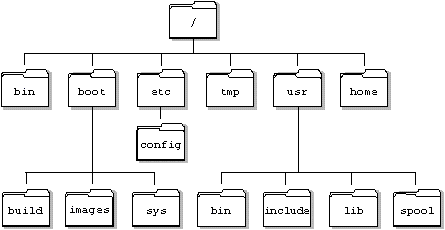
\includegraphics[width=0.6\textwidth]{images/qnx-directory.png}\\
		Image Credit: QNX
	\end{center}



	The directory structure is quite familiar to us as the folders on the system.

	Directories, really, are just like files; they are information about what files are in what locations, and they too will be stored on disk.


\end{frame}

\begin{frame}
	\frametitle{File Operations}

	It makes some sense to consider a file to be a structure.

	A file has some data (fields, metadata).

	There are defined functions, operations to allow users to work with and on files.

\end{frame}

\begin{frame}
	\frametitle{File Operations}
	Six basic operations are required:

	\begin{enumerate}
		\item Creating a file.
		\item Writing a file.
		\item Reading a file.
		\item Repositioning within a file.
		\item Deleting a file.
		\item Truncating a file.
	\end{enumerate}

	Let's examine each of these briefly.

\end{frame}


\begin{frame}[fragile]
	\frametitle{Opening and Closing Files}
	We already saw in an earlier example, one way to open and close a file.
	
	Here is a slight variant that uses \texttt{FILE*}:
	
	\begin{lstlisting}[language=C]
    FILE* f = fopen( argv[1], "r");
    if ( f == NULL ) {
        printf("Unable to open file! %s is invalid name?\n", argv[1] );
        return -1;
    }
    readfile( f );
    fclose( f );
\end{lstlisting}
\end{frame}



\begin{frame}[fragile]
	\frametitle{Using the Open Call}

	It turns out that creating, reading, writing, and truncating involve the open call.

	\begin{lstlisting}[language=C]
FILE * fopen( const char* filename, const char* mode )
\end{lstlisting}

	In addition to the filename as the first parameter, the function is called with the mode as the second parameter.

	In the last example, the mode we provided was a string literal of \texttt{r}.

\end{frame}


\begin{frame}
	\frametitle{Mode Options}

	\begin{itemize}
		\item \texttt{r}
		\item \texttt{w}
		\item \texttt{a}
		\item \texttt{r+}
		\item \texttt{w+}
		\item \texttt{a+}
	\end{itemize}

\end{frame}


\begin{frame}
	\frametitle{More Mode Options}

	If we combine an option with a \texttt{b}, such as \texttt{rb} then we are opening the file as a binary file.

	Also, as of the C 2011 standard, there is a new add-on \texttt{x} which can be used to make any write operation fail if the file exists.

\end{frame}

\begin{frame}
	\frametitle{They Call Me The \texttt{Seek}er}

	Repositioning is also sometimes called a seek operation.

	In C this is done with the \texttt{fseek()} call.

	This adjusts the pointer for reading or writing.

	This should be done with caution though, because you can go to an arbitrary location, even the middle of a two (or more) byte character.

	And we can't seek when a file is opened for append.

\end{frame}


\begin{frame}
	\frametitle{\texttt{DELETE}}

	\begin{center}
		
\includegraphics[width=0.5\textwidth]{images/delete.png}
	\end{center}

\end{frame}


\begin{frame}[fragile]
	\frametitle{Deleting a File}

	In C a file is deleted with the \texttt{remove()} function. This simple program deletes whatever file is provided as the second argument. In reality, we would more likely delete a temporary file that the program has used for some purpose, at the end of execution.

	\begin{lstlisting}[language=C]
int main( int argc, char** argv ) {
  if (argc != 2) {
    return -1;
  }
  
  remove( argv[1] );

  return 0;
}    
\end{lstlisting}

\end{frame}




\begin{frame}
	\frametitle{Combining the Operations}

	These six operations can be combined for most of the other things we may want to do.

	To copy a file, for example, create a new file, read from the old file, and write it into the new file.

	We may also have operations to allow a user to access or set various attributes such as the owner, security descriptors, size on disk...

\end{frame}

\begin{frame}
	\frametitle{Restrictions on the Operations}

	Aside from creation and deletion, all operations are restricted to open files.

	When a file is opened, a program gets a reference to it, and the operating system keeps track of which files are currently open in which process.

	It is good behaviour for a process to close a file when it is no longer using it.

	When the process terminates, that will automatically close any open files (hopefully).

\end{frame}

\begin{frame}
	\frametitle{File Locks}

	Some operating systems support file locks.

	\begin{center}
		
\includegraphics[width=0.2\textwidth]{images/file-lock}
	\end{center}

	Locks may be exclusive, or non-exclusive.

	When a file is locked by one process, other processes will be advised that opening failed due to someone having a lock on that file.

	Similarly, files in use cannot be deleted while that file is in use.

\end{frame}

\begin{frame}
	\frametitle{Windows and UNIX File Locks}

	Windows uses locking; any file that is open in some program cannot be deleted.

	UNIX, however, does not, so UNIX-compatible programs can, if they need, lock a file, but by default this does not happen.

	In UNIX if a file is open in a program, another user can still delete the file and it will be removed from the directory.

	As long as that program remains open and retains that reference to the file, it can still operate on that file.

	However, once the file is no longer open in a program, its storage space will be marked as free.

\end{frame}


\begin{frame}[fragile]
	\frametitle{Locking a File}
	To lock a file in Linux, the call for this is \texttt{flock()}.

	\begin{lstlisting}[language=C]
FILE* f = fopen("myfile.txt", "r");
int file_desc = fileno( f );
int result = flock( file_desc, LOCK_EX );
\end{lstlisting}

	This example locks the file exclusively.

	A shared lock would be \texttt{LOCK\_SH}, and to unlock the parameter is \texttt{LOCK\_UN}.

\end{frame}


\begin{frame}[fragile]
	\frametitle{Writing}

	Writing to a file is easy enough because it works like \texttt{printf}.

	In fact, the function call for it is \texttt{fprintf}.

	The first argument to this is the file pointer where you'd like the data to be written to:

	\begin{lstlisting}[language=C]
void write_points_to_file( point* p, FILE f ) {
  while( p != NULL ) {
    fprintf(f, "(%d, %d, %d)\n", p->x, p->y, p->z);
    p = p->next;
  }
}
\end{lstlisting}
\end{frame}


\begin{frame}[fragile]
	\frametitle{Reading}

	Reading from a file involves the use of \texttt{fscanf} which is a mirror image of \texttt{fprintf}.


	\begin{lstlisting}[language=C]
int main( int argc, char** argv ){
  FILE *fp;
  int i, isquared;
   
  fp = fopen("results.dat", "r");
  if (fp == NULL) {
    return -1;
  }
   
  while (fscanf(fp, "%d,%d\n", &i, &isquared) == 2) {
    printf("i: %d,  isquared: %d\n", i, isquared);
  }
  
  fclose(fp);
  return 0;
}
\end{lstlisting}

\end{frame}



\begin{frame}
	\frametitle{File Types}

	Files we are familiar with often have extensions separated from the file name by a period, like \texttt{fork.txt}.

	The \texttt{txt} extension tells us some information about the file, i.e. it is a text file.

	These things are mostly hints to the OS or user about what sort of file it is.

	In most operating systems, any program can open arbitrary files...

	A \texttt{.docx} extension is only a suggestion that it should be opened by a word processing program.

	OSes typically allow setting a default program for the extension: e.g., always open \texttt{.docx} files with LibreOffice.


\end{frame}

\begin{frame}
	\frametitle{Directories}

	A directory is really just a symbol table that translates file names (user-readable representations) to their directory entries.

	They typically support the operations:

	\begin{enumerate}
		\item \textbf{Search}
		\item \textbf{Add a File}
		\item \textbf{Remove a File}
		\item \textbf{List a Directory}
		\item \textbf{Rename a File}
		\item \textbf{Navigate the File System}
	\end{enumerate}


\end{frame}

\begin{frame}
	\frametitle{Directories}

	There are simple file systems where there are no such things as subdirectories.

	Textbooks may also bring up a structure where each user has his or her own directory but cannot have subdirectories either.

	Tree-structured: there is a root directory, and every file in the system has a unique name when the name and path to it (from the root) are combined.

\end{frame}

\begin{frame}
	\frametitle{UNIX Tree Structured Directory}

	In UNIX the root directory is just called \texttt{/} (forward slash).\\
	\quad From there we can navigate to any file.

	To run the \texttt{ls} command, we will find it in the \texttt{bin} directory as \texttt{/bin/ls}.

	This is an example of an absolute path.

\end{frame}

\begin{frame}
	\frametitle{UNIX Tree Structured Directory}

	Most of the time we do not have to use the absolute path (the full file name); a relative path (the path from the current directory) will suffice.

	Example: compile something with a command like \texttt{gcc code/example.c}.

	The file \texttt{example.c} is in a subdirectory of the current directory called \texttt{code}.

	The system will work out that we need to start from the current directory (e.g., \texttt{/home/jz/ece252/}) and prepend that to the given file name.

	This produces the absolute path of \texttt{/home/jz/ece252/code/example.c}.

\end{frame}



\begin{frame}
	\frametitle{Deleting a Directory}

	What if a directory is not empty?

	If it is empty, just removing the directory is enough.

	If it contains some files, either the system can refuse to delete the directory until it is empty, or automatically delete the files and subdirectories.

\end{frame}

\begin{frame}
	\frametitle{Deletion}

	Also, what does it mean to delete a file or folder?

	The delete command sometimes does not necessarily actually delete the file or folder, but instead moves it to some deleted files directory.

	If it is deleted from there then it is really gone, but while it is in that deleted file directory it can be restored.

\end{frame}

\begin{frame}
	\frametitle{Sharing of Files}

	File systems may also support the sharing of files.

	There is one copy of the file but it has more than one name.

	In UNIX this is called a \alert{link} and this is effectively a pointer to another file.

	Links are either ``hardlinks'' or ``symlinks''.

\end{frame}

\begin{frame}
	\frametitle{Symbolic Links}

	Symlinks, or symbolic links, are just references by file name.

	So if a symbolic link is created to a file like \texttt{/Users/jz/file.txt}, the symbolic link will just be a ``shortcut'' to that file.

	If the file is later deleted, the symbolic link is left pointing to nothing.

	A future attempt to use this pointer will result in an error.

	It would be expensive, though possible, to search through the file system to find all links and remove them.


\end{frame}

\begin{frame}
	\frametitle{Hard Links}

	Creating a hardlink is creating a pointer to the underlying file in the file system.

	If a hardlink exists and the user deletes that file, the file still remains on disk until the last hardlink is removed.

	The file structure maintains a count of how many hardlinks reference a file, and it is only really deleted if the count falls to zero.


\end{frame}



\begin{frame}
	\frametitle{File Permissions}

	Files usually have some permissions associated with them:

	\begin{enumerate}
		\item Read
		\item Write
		\item Execute
		\item Append (write at the end of the file)
		\item Delete
		\item List (view the attributes of the file)
	\end{enumerate}

\end{frame}

\begin{frame}
	\frametitle{Access Control: UNIX-Style}

	These are used often in UNIX(-like) systems.

	Each file has an owner and a group.

	Permissions can be assigned for the:
	\begin{itemize}
		\item Owner
		\item Group
		\item Everyone
	\end{itemize}


\end{frame}

\begin{frame}
	\frametitle{Access Control: UNIX-Style}


	There are three basic permissions:

	\begin{itemize}
		\item Read
		\item Write
		\item Execute
	\end{itemize}

	Permissions are represented by 10 bits:\\
	\quad 1 indicates true and 0 indicates false.

	First bit is the directory bit.

	Next three are read, write, execute for the owner.\\
	Then read, write, execute for the group.\\
	Finally, read, write, execute for everyone.


\end{frame}

\begin{frame}
	\frametitle{Access Control: UNIX-Style}


	The permissions can be shown in a human-readable format.

	The order is always the same, and so a dash (\texttt{-}) appears if a bit is zero (permission does not exist).

	The character \texttt{d} is used to indicate a directory.

	\texttt{r} to indicate read access.

	\texttt{w} to indicate write access.

	\texttt{x} to indicate execute access.



\end{frame}

\begin{frame}
	\frametitle{Access Control: UNIX-Style Example}


	Example: \texttt{-rwxr{-}{-}{-}{-}{-}}

	This means:
	\begin{itemize}
		\item not a directory;
		\item the owner can read, write, and execute;
		\item other members of the group can read it only
		\item everyone else has no access to the file (cannot read, write, or execute).
	\end{itemize}


\end{frame}

\begin{frame}
	\frametitle{Access Control: UNIX-Style}


	Permissions can also be written in octal (base 8): \\
	\quad r = 4, w = 2, and x = 1.

	Start with 0, and then add the value of the  permissions that are present, using zero where permissions are absent.

	Example: \texttt{750} \mnote{meaning that the owner has read, write and execute access (0 + 4 + 2 + 1 = 7); group members have read and execute access (0 + 4 + 0 + 1 = 5); everyone else has no access to it at all.}


\end{frame}

\begin{frame}
	\frametitle{Access Control: UNIX-Style}


	More details: like what the permissions mean on directories,

	Advanced topics like \texttt{setuid}, \texttt{setgid}, and ``sticky bit''.

	Beyond the scope of this course.


\end{frame}

\begin{frame}
	\frametitle{Access Control: UNIX-Style}


	The obvious shortcoming: very coarse grained.

	Another strategy is used by SELinux and Windows NT: ACLs.

	... But we will consider that beyond the scope of the course for now.
\end{frame}

\end{document}

